In this section, we will explore the machine learning techniques utilized
in this study. Initially, we will delve into convolutional neural networks
(CNNs) and their advantages compared to multilayer perceptrons (MLPs).
Following the introduction of CNNs, we will focus U-Net a widely used fully convolutional network architecture.
Additionally, we will examine LSTM networks and their extension to ConvLSTM that incorporates convolutions.
\medskip

\subsection{Convolutional Neural Networks}

Convolutional neural networks (CNNs) were initially introduced by Yann LeCun in 1998 and applied to the challenge of handwritten digit classification \cite{lecun-1998}. However, the breakthrough for CNNs came later with the remarkable success achieved by Krizhevsky et al. in the ImageNet paper of 2012. This pivotal work revolutionized the field of image classification by significantly advancing the state of the art on the ImageNet dataset \cite{krizhevsky-2017}.

CNNs are a class of deep learning models strongly capable of solving computer vision tasks. Unlike fully connected neural networks, which treat input data as a one dimensional vector, CNNs are designed to process higher dimensional data such as images.
This distinction enables CNNs to exploit more spatial relationships and patterns in visual data as opposed to a flattened vector where these patters are not recoverable.

Additionally Convolutional neural networks reduce the amount of parameters that are needed for each layer. This reduction is caused by parameter sharing, in a
traditional multi-layer perceptron weights exist for each connection while in CNNs a set of kernels are applied to the input. The kernels used in CNNs are small and repeatedly applied across the input.
This reduces the amount of parameters the network has. 

\begin{figure}
  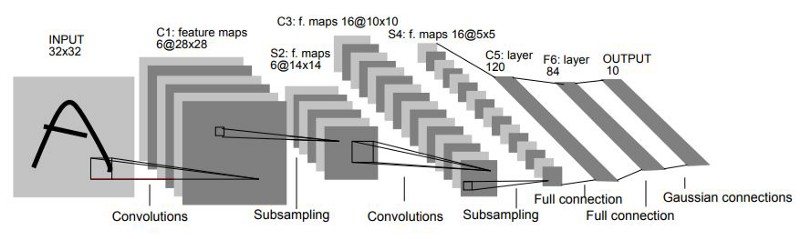
\includegraphics[width=8cm]{../images/cun.jpeg}
  \caption[short]{Architecture of LeNet-5: used for digit recognition and introduced by Yan LeCun \cite{lecun-1998}}
\end{figure}

\subsection{U-Net}
Semantic segmentation, the task of assigning a class label to each pixel in an image, is key to understand an image from a computer vision perspective.
This is the starting point for U-Net which was developed by Ronneberger et al. \cite{ronneberger-2015} to segment images from microscopes in biomedical applications.
U-Net is a fully convolutional architecture that provides accurate and detailed pixel-level predictions.
The U-Net architecture is specifically designed to capture both local and global context information.
The U-Net architecture gets its name from its U-shaped design (Figure \ref{fig:unet}), which consists of an encoder path and a decoder path.
The encoder path resembles a traditional CNN and serves to capture spatial information and learn feature representations at various scales.
It typically comprises multiple convolutional and pooling layers, where each convolutional layer extracts increasingly abstract features by convolving with learnable filters and applying non-linear activation functions.
The decoder path, on the other hand, aims to recover the spatial information lost during the pooling and down-sampling operations of the encoder.
It employs a series of upsampling and transposed convolutional layers to gradually increase the spatial resolution and reconstruct the detailed predictions.
The skip connections between the corresponding encoder and decoder layers help preserve fine-grained details and enable the fusion of local and global context information, facilitating more accurate segmentation.
These skip connections bridge the gap between low-level and high-level features, allowing the network to leverage both local and global context for precise pixel-wise predictions.
One of the key advantages of U-Net is its ability to capture contextual information effectively. By using skip connections, the network can combine low-level and high-level features, enabling the model to refine predictions by incorporating local details and global context simultaneously. This property is especially beneficial for tasks like semantic segmentation, where precise boundary delineation and accurate classification of object categories are essential.
\begin{figure}
  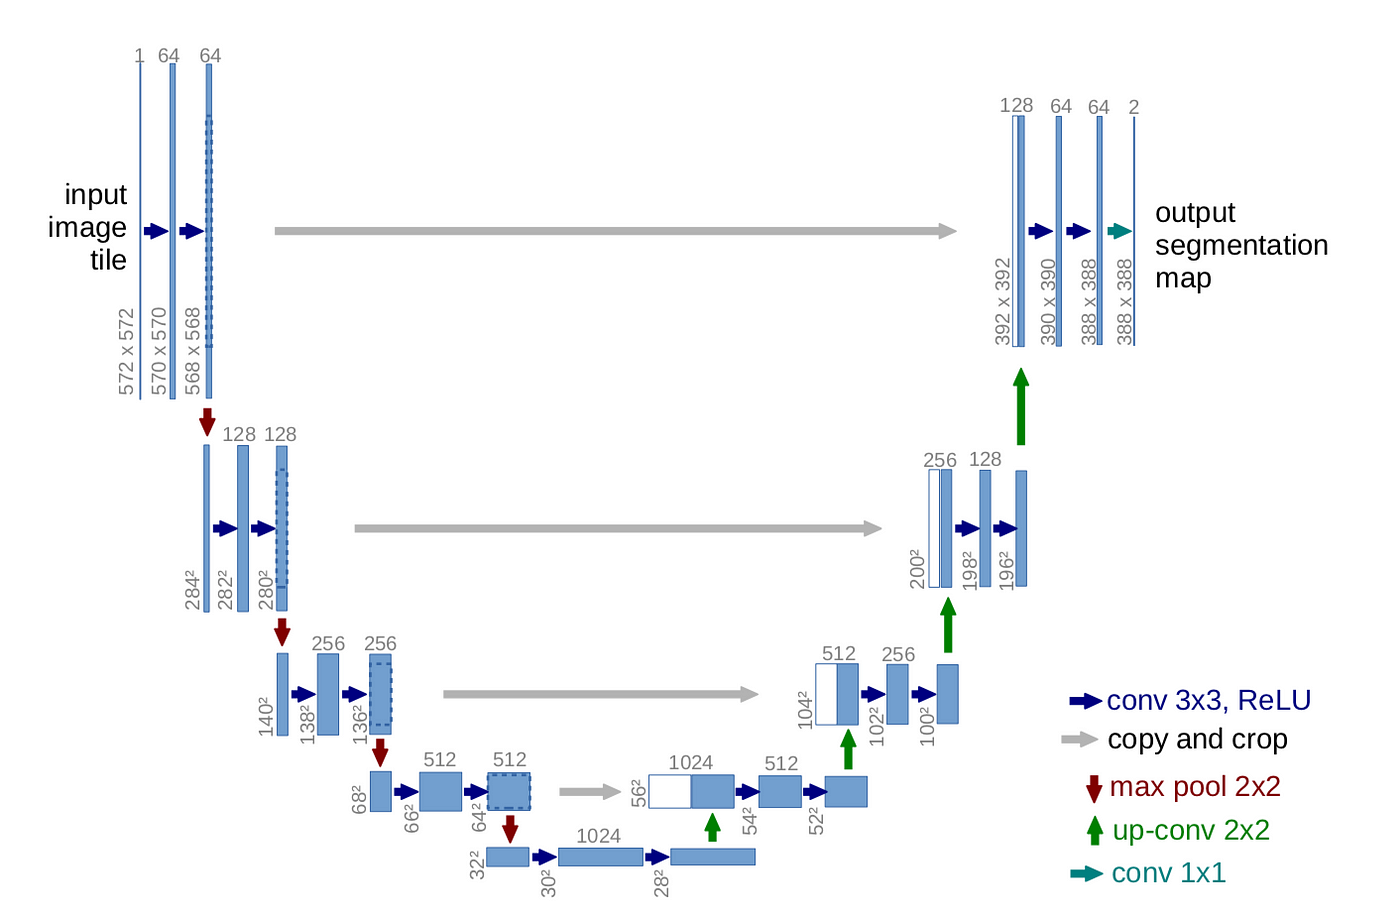
\includegraphics[width=8cm]{../images/unet.png}
  \caption[short]{U-Net}
  \label{fig:unet}
\end{figure}

\subsection{Convolutional LSTM}

\subsection{Attention}
Designed for machine translation Bahadanau et al. can be applied to sequence to sequence encoder decoder models.
how to pay the right amount of attention to the input sequence.